\begin{questionS}
Write a function
\begin{scala}
  def qSort(in: ??[Int], out: !![Int]): ThreadGroup
\end{scala}
that receives a stream of data on |in|, and outputs a sorted version on~|out|.
The sorting should be done using the Quicksort algorithm.  In the case that
the input stream contains at least one value, starting with a value~|pivot|,
use two recursive calls to |qSort| to sort the values that are less
than~|pivot|, and the other values that are greater than or equal to~|pivot|,
respectively.

Test your code. 
\end{questionS}

%%%%%%%%%%%%%%%%%%%%%%%%%%%%%%%%%%%%%%%%%%%%%%%%%%%%%%%

\begin{answerS}
My code is below.  I use an |attempt| structure to deal with the case that the
input stream is empty.  Otherwise, I build the system below, with two
recursive calls to |qSort|, and a controller tying them together.
%
\begin{center}
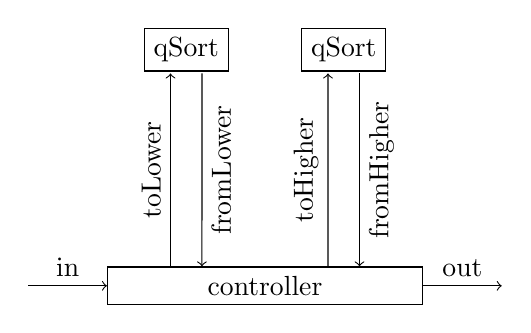
\begin{tikzpicture}
\draw (0,0) node[draw, minimum width=40mm] (controller) {\scalashape controller};
\draw[->] (controller.west) ++ (-1,0) -- 
   node[above]{\scalashape in} (controller.west);
\draw[<-] (controller.east)++(1,0)  -- 
   node[above]{\scalashape out} (controller.east);
%
\draw (controller) ++ (-1,3) node[draw] (rec1) {\scalashape qSort};
\draw (rec1.south)++(-0.2,0.1) node (rec1In) {};
\draw[->] (controller.north) ++ (-1.2,0.0) -- 
  node[above,sloped] {\scalashape toLower} (rec1In);
\draw (rec1.south)++(0.2,0.1) node (rec1Out) {};
\draw[<-] (controller.north) ++ (-0.801,0) -- 
  node[below,sloped] {\scalashape fromLower} (rec1Out);
%
\draw (controller) ++ (1,3) node[draw] (rec2) {\scalashape qSort};
\draw (rec2.south)++(-0.2,0.1) node (rec2In) {};
\draw[->] (controller.north) ++ (0.8,0.0) -- 
  node[above,sloped] {\scalashape toHigher} (rec2In);
\draw (rec2.south)++(0.2,0.1) node (rec2Out) {};
\draw[<-] (controller.north) ++ (1.2,0) -- 
  node[below,sloped] {\scalashape fromHigher} (rec2Out);
\end{tikzpicture}
\end{center}
%
The controller distributes input values to the two sub-sorters, depending on
how it compares with~|pivot|.  When the input stream is closed, it closes its
channels to the sub-sorters, to indicate that their input streams are
finished.  It then takes outputs from the two sub-sorters, and passes it out,
together with |pivot|, in the right order.
%
\begin{scala}
  def qSort(in: ??[Int], out: !![Int]): ThreadGroup = thread("QSort"){
    attempt{
      val pivot = in?()
      val toHigher, toLower, fromHigher, fromLower = new SyncChan[Int]
      // Controller thread.
      def controller = thread("Controller"){
	// Split data received on £in£ between £higher£ and £lower£, depending on
	// whether it is £$\ge \sm{pivot}$£ or £$< \sm{pivot}$£, respectively.
	repeat{ val x = in?(); if(x < pivot) toLower!x else toHigher!x }
	// We've received the final input, so close the channels to the
	// sub-sorters.
	toHigher.endOfStream(); toLower.endOfStream()
	// Now output the results.
	repeat{ out!(fromLower?()) }; out!pivot; repeat{ out!(fromHigher?()) }
	out.endOfStream()
      }      
      // Put the system together, and run it.
      run(controller || qSort(toHigher, fromHigher) || qSort(toLower, fromLower))
    }{ out.endOfStream() } // We've received no data, so just close.
  }
\end{scala}
\end{answerS}
